\documentclass[]{article}
\usepackage[utf8]{inputenc}
\usepackage[english]{babel}
\usepackage{graphicx}
\usepackage{float}
\date{\vspace{-5ex}}
\graphicspath{{./images/}}
\usepackage{hyperref}
\hypersetup{
	colorlinks,
	citecolor=black,
	filecolor=black,
	linkcolor=blue,
	urlcolor=blue
}
%opening
\title{Proposal for Google Summer of Code: Procedural animation implementation for Godot Engine}
\author{Yael Atletl Bueno Rojas}

\begin{document}

\maketitle

\begin{abstract}
	This system will be based on the GDC talk: “Animation Bootcamp, an indie approach to procedural animation”, reducing animation workload. 

\end{abstract}

\tableofcontents
\newpage
\section{Personal information}
\subsection{Contact information}
\begin{itemize}
\item[E-mail:] \href{mailto:yael.atletl@gmail.com}{yael.atletl@gmail.com} 
\item[Discord:] 810-dude\#9229
\item[Matrix:] @biodude:matrix.org
\item[Location:] Puebla, Mexico
\item[Timezone:] UTC-6
\end{itemize}
\subsection{Background}
I am a second semester computer science student from the Benem\'erita Universidad Aut\'onoma de Puebla, I have been developing various projects with Godot since 2017, one being \href[]{https://github.com/RiseRobotRise/Joyeuse/}{a framework} for creating shooters and some community games. I have developed \href[]{https://github.com/yaelatletl}{other side projects} and worked as a programmer for \href[]{https://github.com/briligg/Moonwards-Virtual-Moon}{Moonwards} for 4 months. 
You can also see I have summited issues to the Godot github page in \href[]{https://github.com/godotengine/godot/issues/created_by/yaelatletl}{this link}.

\section{Project description}
Create a system that will allow developers to visually edit and mix procedural animations. This will be archived using two new resources: ProceduralAnimation and PoseLibrary. It will be usable with AnimationPlayer or AnimationPlayerTree. It will use a special editor for this animations and could be used the same way normal animations are used. 

For a better result, blend spaces should be used. 
An example project will be made for illustrating how to use this along with other systems already on Godot to obtain fluid animations. To be made as reusable as possible so anyone can just base their project on the demo. 

\subsection{ProceduralAnimation}
The resource will behave as an Animation resource codewise and will be usable in either an animation player or an animation tree.

A process is described for creating a Procedural Animation:
\begin{enumerate}
\item The User is asked to select an animation to use as pose library. (This will create and load a PoseLibrary)
\item Each keyframe will be used as a pose and will be stored in a PoseLibrary resource
\item The user will be able to select which and how many poses to use, adding and deleting them on the fly, will also be able to change the animation time. 
\item Poses will be able to be mirrored when the bones on the skeleton are labeled like this: L\_leg, R\_leg, L\_arm, R\_arm, etc. 
\item A connection graph will be placed between two poses,giving three options for interpolating the poses: 
\begin{itemize}
\item Linear.
\item Bicubic (default).
\item Discrete (along with linear, may be useful for animations in stop-motion style).
\end{itemize}

\item The animation will by default space evenly the keyframes in the animation time.
\item Poses will be then placed in a timeline with an identifier so the user can tweak timing.
\end{enumerate}

\begin{figure}[H]
	\centering
	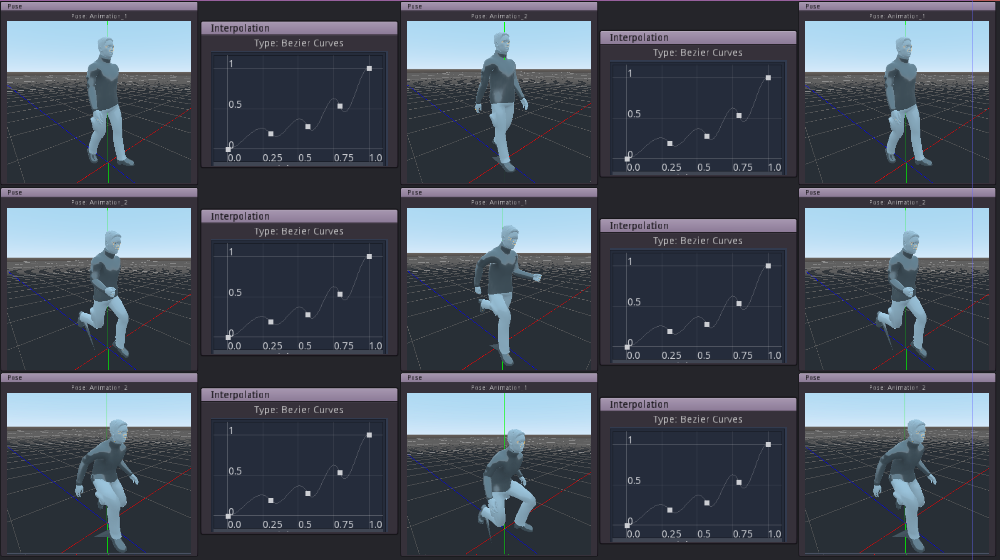
\includegraphics[width=1\textwidth]{mockup}
	\caption{Concept for various animations, curves here are just an example.}
\end{figure}

\subsection{PoseLibrary}
The resource should be used under the same concept as a libmesh. It contains single frames with thumbnails so the user can use them on a ProceduralAnimation.

\subsection{Demo project}
This will be a character in a simple scenario, it will be able to walk, run, crouch walk and jump and when a key is pressed it will enter ragdoll mode.
For animations will use blendspaces with ProceduralAnimation; for secondary movement, an antenna and a cape are to be used as an example. 
Implementing foot matching the floor is a stretch goal. 

For this project, PoseLibrary and Blend files are to be included. 

\section{Use case}

Procedural animation, as shown in the GDC talk this proposal is based on, reduces the workload of animators and gives a fluid look to animations as it provides more control over how the poses are transitioned. 

The demo project will allow newcomers and established users to understand how to bring to life their characters in Godot. 

\section{Motivation}

I started back in 2017 to use Godot, all through early builds and an alpha, it didn’t take me too long to get used to working with Godot as my main tool, even if I had came from a different kind of environment, where tools were simple and pretty easy to use, but were limited, buggy and had no way to go further. The change in the way I can actually contribute to the engine I use really helped me get my ideas clear. I don’t want to just use what’s already there and build workarounds for myself. I want to give everyone better tools for making games, the tools I wish I started with, so I wish to contribute to make a great tool an even better tool. 

\section{Initial Research}

As the base for this proposal is  \href[]{https://www.youtube.com/watch?v=LNidsMesxSE}{this video} most of the research was done from there.

For procedural animation, the most common topics are: 
\begin{itemize}
\item Ragdolls.
\item Animation Tree Matching.
\item Pose transitioning using curves.
\item Inverse Kinematics (Tracking and refining).
\item Secondary motions (Physics simulated).
\end{itemize}


Some of these are already in godot:
\begin{itemize}
\item	Ragdolls (since 3.1).
\item	Inverse Kinematics for tracking.
\item	Secondary motions (Cloth simulation and \href[]{https://github.com/Bauxitedev/godot-jigglebones}{jiggle bones}).
\end{itemize}


This leaves only some things to be implemented:
\begin{itemize}
\item Animation Tree Matching.
\item Pose transitioning using curves (This proposal). 
\item Inverse Kinematics for refining (could  \href[]{https://www.youtube.com/watch?v=MonxKdgxi2w}{be ported}).
\end{itemize}


\section{Aproximate timeline }
\begin{itemize}
	
\item [Pre GSoC] Learning to modify the source code, adapting to the workflow and bonding with community.

\item [Week 1-3] Implement the pose library resource and a way to generate it from the animation player editor.

\item [Week 4-6] Implement the ProceduralAnimation editor and resource, instead of just generate a Poselib open an editor.

\item [Week 7-9] Bug-fixing and refinement. 

\item [Week 9-12] Work on the Demo Project, integrate as many animation related things already on Godot as possible.   
\end{itemize}

\end{document}
